\bf{Example}

Let $N=4,$ $M=4,$ $U=[0,0,0,1],$ $V=[1,2,3,2],$ $A=1,$ $B=3,$ $S=1,$ and $T=3.$

The grader calls \t{find_pair(4, [0, 0, 0, 1], [1, 2, 3, 2], 1, 3).}

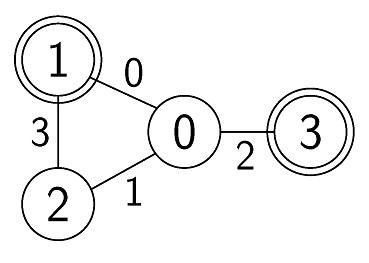
\includegraphics{image0.jpg}

In the figure above, the edge with number i corresponds to the highway i. Some possible calls to \t{ask} and the corresponding return values are listed below:

\begin{tabular}{|c|c|} \hline
\bf{Call}&\bf{Return} \\\hline
\t{ask([0, 0, 0, 0])}&$2$ \\\hline
\t{ask([0, 1, 1, 0])}&$4$ \\\hline
\t{ask([1, 0, 1, 0])}&$5$ \\\hline
\t{ask([1, 1, 1, 1])}&$6$ \\\hline
\end{tabular}

For the function call \t{ask([0, 0, 0, 0])}, the traffic of each highway is light and the toll for each highway is $1.$ The cheapest route from $S=1$ to $T=3$ is $1 \rightarrow 0 \rightarrow 3.$ The total toll for this route is $2.$ Thus, this function returns $2.$

For a correct answer, the procedure \t{find_pair} should call \t{answer(1, 3)} or \t{answer(3, 1)}.

The file \t{sample-01-in.txt} in the zipped attachment package corresponds to this example. Other sample inputs are also available in the package.

